A Figura \ref{fig:altitude_z_zdot_2kg} mostra a posição no eixo vertical ($z$) do \textit{drone}, bem como sua variação no sistema em que atua o controlador \textit{fuzzy} projetado. Como se pode ver, o distúrbio foi devidamente controlado, fazendo com que o quadricóptero retornasse à posição inicial $z=-2$ m e também ao repouso\footnote{i.e.\ velocidade nula} representado por $\dot{z}=0$ m/s. Nesta figura, entretanto, não fica tão clara a diferença de desempenho dos controladores \textit{fuzzy} e neuro-\textit{fuzzy}, aspecto que pode ser claramente verificado na Figura \ref{fig:altitude_z_zdot_2kg_closer}. Como se pode ver, tanto para $z$ quanto para $\dot{z}$, o neuro-\textit{fuzzy} apresenta desempenho melhor. No controle sobre a posição $z$, o controlador neuro-\textit{fuzzy} apresentou redução do tempo de convergência em 29\%, e da variação do sistema em 31\%, além de eliminar a sobrelevação apresentada pelo \textit{fuzzy}. Já sobre a velocidade $\dot{z}$, apresentou uma redução no tempo de convergência de 29\% além melhorar a variação do sistema em 23\%. A partir destes resultados, verifica-se que o controlador neuro-\textit{fuzzy} fez com que o distúrbio fosse melhor absorvido e que sua correção ocorresse mais rapidamente.

% Altitude m=2
\begin{figure}[!htb]
    \centering
    \caption{Comparação da resposta das saídas $z$ e $\dot{z}$ no controle de altitude \textit{fuzzy} e neuro-\textit{fuzzy} para o sistema com massa $m=2$ kg}
    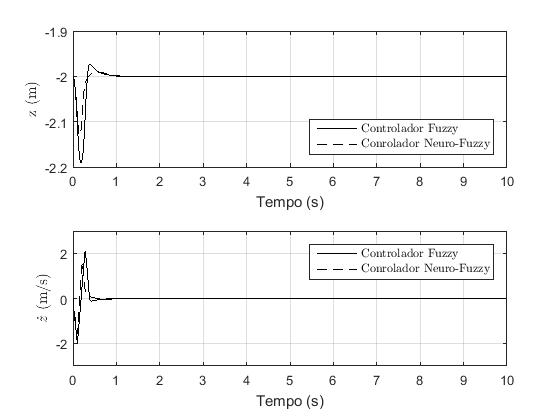
\includegraphics[width=0.8\textwidth]{./04-figuras/figuras_pos_banca/5-altitude2kg/graph_z_zdot_2kg}
    \label{fig:altitude_z_zdot_2kg}
\end{figure}

% Altitude m=2, closer
\begin{figure}[!htb]
    \centering
    \caption{Comparação em mais detalhes da resposta das saídas $z$ e $\dot{z}$ no controle de altitude fuzzy e neuro-fuzzy para o sistema com massa $m=2$ kg}
    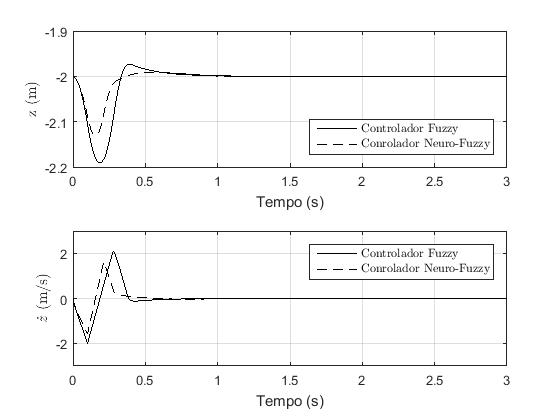
\includegraphics[width=0.8\textwidth]{./04-figuras/figuras_pos_banca/5-altitude2kg/graph_z_zdot_2kg_details}
    \label{fig:altitude_z_zdot_2kg_closer}
\end{figure}

% -------------------  ATITUDE ---------------

Já as Figuras \ref{fig:atitude_phi_phidot_2kg_40s} e \ref{fig:atitude_theta_thetadot_2kg_40s} mostram a estabilidade de atitude em torno dos eixos x e y (i.e\ em relação ao plano horizontal XY), representados por $\theta$ e $\phi$ respectivamente. Como se pode ver, ambos os estados são devidamente controlados e, com isto, o quadrotor volta à estabilidade horizontal, com ângulos e velocidades angulares nulas no estado permanente.

% Atitude m=2
%phi
\begin{figure}[!htb]
    \centering
    \caption{Comparação da resposta das saídas $\phi$ e $\dot{\phi}$ no controle de atitude fuzzy e neuro-fuzzy para o sistema com massa $m=2kg$}
    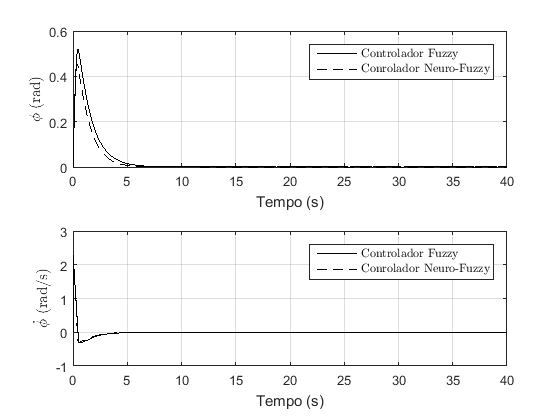
\includegraphics[width=0.8\textwidth]{./04-figuras/resultados/novos/atitude_phi_phidot_2kg_40s}
    \label{fig:atitude_phi_phidot_2kg_40s}
\end{figure}

%theta
\begin{figure}[!htb]
    \centering
    \caption{Comparação da resposta das saídas $\theta$ e $\dot{\theta}$ no controle de atitude fuzzy e neuro-fuzzy para o sistema com massa $m=2kg$}
    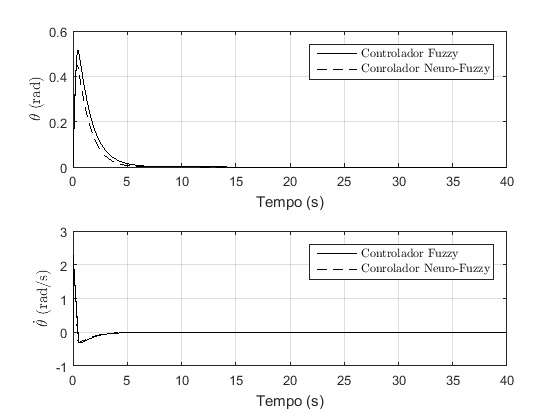
\includegraphics[width=0.8\textwidth]{./04-figuras/resultados/novos/atitude_theta_thetadot_2kg_40s}
    \label{fig:atitude_theta_thetadot_2kg_40s}
\end{figure}

A partir das Figuras \ref{fig:atitude_phi_phidot_2kg_10s} e \ref{fig:atitude_theta_thetadot_2kg_10s}, que mostram as respostas obtidas em mais detalhes, pode-se ver que, mais uma vez o controlador neuro-fuzzy mais uma vez teve desempenho superior ao fuzzy, fazendo com que os ângulos $\phi$ e $\theta$ convergissem 2\% mais rápido, além de reduzir suas variações em 13\%. Com relação às velocidades angulares $\dot{\phi}$ e $\dot{\theta}$, foi capaz de reduzir o tempo de convergência em 3\%, não afetando a variação nem a sobrelevação apresentada pelo sistema quando estabilizado pelo controlador fuzzy. Desta forma, verifica-se que o controle neuro-fuzzy levou o sistema a uma menor variação, representando que o ângulo máximo de inclinação alcançado pelo drone é menor e corrigido mais rapidamente.

\begin{figure}[!htb]
    \centering
    \caption{Comparação em mais detalhes da resposta das saídas $\phi$ e $\dot{\phi}$ no controle de atitude fuzzy e neuro-fuzzy para o sistema com massa $m=2kg$}
    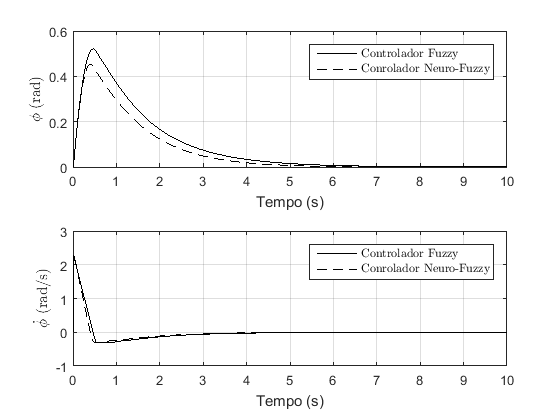
\includegraphics[width=0.8\textwidth]{./04-figuras/resultados/novos/atitude_phi_phidot_2kg_10s}
    \label{fig:atitude_phi_phidot_2kg_10s}
\end{figure}

%theta
\begin{figure}[!htb]
    \centering
    \caption{Comparação em mais detalhes da resposta das saídas $\theta$ e $\dot{\theta}$ no controle de atitude fuzzy e neuro-fuzzy para o sistema com massa $m=2kg$}
    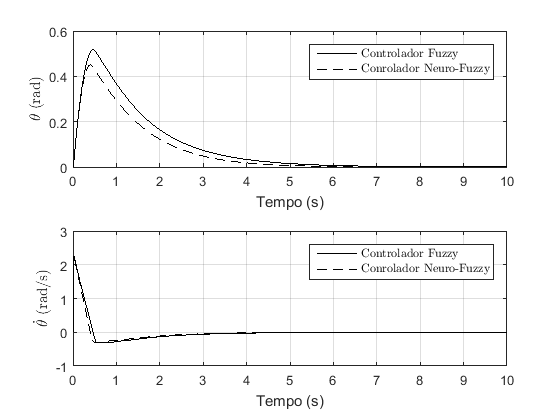
\includegraphics[width=0.8\textwidth]{./04-figuras/resultados/novos/atitude_theta_thetadot_2kg_10s}
    \label{fig:atitude_theta_thetadot_2kg_10s}
\end{figure}